% ch_integer_programming.tex  —  Chapter: Integer programming: binary decisions in fleet renewal and retrofit
% Content only — compiled via main.tex
% Figures in fig/, code in code/
\chapter{Integer programming: binary decisions in fleet renewal and retrofit}
\label{ch:ip-intro}

The previous chapter treated every decision variable as continuous, such as a
cargo quantity, or a number of cabins. These could take any non-negative real
value. \emph{Divisibility} was one of the four defining assumptions of a
linear program, and we saw in the cabin
problem that an integer-valued optimum can appear in a continuous LP
purely by coincidence (and thus, no integer-specific constraints are needed). 
However, we cannot generally assume this for any arbitrary discrete design problem. 
In particular for yes/no problems, such as whether to install a particular retrofit package on a
particular vessel, whether to build a salmon farm at one location or two, whether
a given tank position holds one product type or another. Modelling them as continuous variables that happen to
settle at $0$ or $1$ is not a strategy that can be relied on.

This chapter introduces \emph{integer programming}, and its most common
special case, \emph{binary integer programming}, as the natural extension
of the LP problem, with a focus on discrete decisions.
Section~\ref{sec:binary-modelling} develops a small toolbox of binary
modelling constructs --- mutually exclusive choices, conditional
decisions, and installation--use linkages --- that recur throughout ship
design optimization. Section~\ref{sec:knapsack} applies this toolbox to
the classical knapsack problem, introducing the central practical concern
of this chapter: a correct formulation is not automatically a good one,
and some formulations solve far more easily than others.
Section~\ref{sec:bnb} develops branch-and-bound, the exact solution method
underlying every commercial and open-source MILP solver, including
Xpress. Section~\ref{sec:fleet-retrofit} brings all of this together in a
single, sizeable worked example: choosing which emission-abatement
retrofits to install, on which vessel, and when, to meet a
stepwise-tightening fleet emissions cap at minimum cost --- the fleet
renewal and retrofit problem that anchors assignment A4.

\section{From continuous to discrete decisions}
\label{sec:ip-intro-sec}

\subsection{Where the linear program breaks down}

A number of cabins, an on/off retrofit decision, or a choice between two
candidate factory sites is not a divisible quantity: $x=0.4$ of a
heat-recovery unit installed is not a meaningful design. When a decision
variable is restricted to take only integer values --- or, in the common
special case of a yes/no decision, only the values $0$ and $1$ --- the
resulting problem is an \emph{integer program}. Everything else about the
model is unchanged: objective and constraints remain linear in the
decision variables, so the structured formulation discipline developed for
linear programs (sets, parameters, variables, model) applies without
modification. Only the domain of the variables changes.

\subsection{Pure, mixed, and binary integer programs}
\label{sec:ip-types}

It is useful to distinguish three variants, since the terminology recurs
throughout the literature and in solver documentation.

\begin{description}
  \item[(Pure) integer programming, IP.] All decision variables are
  restricted to integers, $x_j \in \mathbb{Z}_{\geq 0}$.
  \item[Mixed integer programming, MIP.] Some variables are restricted to
  integers, others remain continuous. Most realistic ship design models
  are of this type: a design decision might be integer (number of tanks)
  while an associated operating quantity remains continuous (tonnes of
  product carried in each tank).
  \item[Binary integer programming, BIP.] Every integer variable is
  further restricted to $\{0,1\}$. This is overwhelmingly the most common
  case in design and configuration problems, because most genuinely
  discrete design decisions are yes/no choices at the level the model
  represents them.
\end{description}

A general mixed-integer linear program can be written
\begin{align}
  \max \quad & Z = \sum_{j=1}^{n} c_j x_j \notag\\
  \text{s.t.} \quad & \sum_{j=1}^{n} a_{ij}x_j \leq b_i, \quad i=1,\ldots,m \notag\\
  & x_j \geq 0, \quad j=1,\ldots,n \notag\\
  & x_j \in \mathbb{Z}, \quad j \in J \subseteq \{1,\ldots,n\}, \notag
\end{align}
where $J$ is the subset of variables restricted to integers ($J=\{1,\ldots,n\}$
for a pure IP, and $x_j \in \{0,1\}$ for $j\in J$ for a BIP).

\subsection{The LP relaxation}
\label{sec:lp-relaxation}

Dropping the integrality restriction on every $x_j\in J$ and solving the
resulting ordinary linear program is called the \emph{LP relaxation} of
the integer program. Because the LP relaxation is solved over a
\emph{larger} feasible region than the original problem (every
integer-feasible point is also LP-feasible, but not vice versa), its
optimal value is always at least as good as the integer program's --- an
upper bound for a maximization problem, a lower bound for a minimization
problem. This bounding property is the single most important tool in
solving integer programs, and underlies the branch-and-bound method of
Section~\ref{sec:bnb}.

It also explains an apparent paradox: an integer program is, for equal
numbers of variables and constraints, almost always \emph{harder} to
solve than its LP relaxation, even though it has \emph{fewer} feasible
points. Removing points from a feasible region does nothing to make a
linear program's own structure --- convexity, the guarantee that an
optimum sits at a vertex --- any easier to exploit; it only removes the
guarantee that the Simplex method's vertex-to-vertex search will land on
a feasible point at all. Solving an integer program therefore generally
means solving \emph{many} LP relaxations, not one. (There are well-known
exceptions: the transportation problem introduced later in the course
happens to have an LP relaxation whose optimal basic solutions are
automatically integer, for any integer supply and demand data --- a
property of that particular constraint structure, not something to expect
in general.)

\section{Modelling logical relationships with binary variables}
\label{sec:binary-modelling}

A binary variable $\delta_k\in\{0,1\}$ is most useful not as a quantity
but as an \emph{indicator}: $\delta_k=1$ if some discrete choice $k$ is
made, $\delta_k=0$ otherwise. A small number of linear constraint patterns,
combined, can express most of the logical relationships that arise
between such choices. Table~\ref{tab:binary-constructs} collects the
constructs used repeatedly in this chapter and in the term project; in
each case $x_A,x_B\in\{0,1\}$ are indicators for decisions $A$ and $B$.

\begin{table}[htbp]
  \centering
  \caption{Standard binary modelling constructs.}
  \label{tab:binary-constructs}
  \begin{tabular}{@{}p{0.27\textwidth}p{0.22\textwidth}p{0.4\textwidth}@{}}
    \toprule
    Relationship & Constraint & Ship design example \\
    \midrule
    At most one of $A,B$ (mutually exclusive) & $x_A+x_B\leq 1$ & Build the salmon fodder factory at Fr{\o}ya \emph{or} Bjugn, not both \\
    At most $k$ of $n$ options & $\sum_{k} x_k \leq k^{\max}$ & Install at most two of the four available retrofits \\
    Exactly one of $n$ options (partition) & $\sum_{k} x_k = 1$ & Choose exactly one propulsion configuration \\
    $A$ implies $B$ (``if $A$ then $B$'') & $x_A - x_B \leq 0$ & If a propeller is fitted, a shaft must be too \\
    $B$ only if $A$ (converse implication) & $x_B - x_A \leq 0$ & An abatement option is only in use if it has been installed \\
    $A$ and $B$ logically equivalent & $x_A = x_B$ & Installation and use coincide exactly \\
    \bottomrule
  \end{tabular}
\end{table}

The last two rows are easy to confuse: ``$A$ implies $B$'' and ``$B$ only
if $A$'' are converse statements, and the correct constraint direction
depends on which one is meant. A useful check is to ask which combination
is being ruled out: $x_A-x_B\leq0$ rules out $x_A=1,x_B=0$ (installing $A$
without $B$); $x_B-x_A\leq0$ rules out $x_B=1,x_A=0$ (using $B$ without
$A$ ever having been installed). Section~\ref{sec:fleet-retrofit} uses
exactly this second pattern to tie the use of an abatement option to its
installation.

A related and very common construct links a binary decision to a
continuous or bounded quantity: ``if $\delta=0$ then $y=0$'' is enforced
by $y\leq M\delta$ for a suitably large constant $M$ (a \emph{big-M}
constraint). This is often unavoidable, but it comes at a cost: the LP
relaxation of $y\leq M\delta$ allows $y$ to be as large as $M\delta$ for
any fractional $\delta$, which can be costly for the
branch-and-bound algorithm. Thus choosing the smallest possible
$M$ --- or, where possible, avoiding the construct altogether in favour of
an exact algebraic relationship --- is often a better solution.
Section~\ref{sec:fleet-retrofit} describes a case where a
big-M constraint used in an existing model turns out to be unnecessary,
and removing it tightens the LP relaxation substantially.

\section{The 0/1 knapsack problem}
\label{sec:knapsack}

\subsection{Formulation}

The \emph{0/1 knapsack problem} is the simplest genuine binary integer
program, and a useful reference point before tackling larger models:
choose a subset of $n$ available items, each with a value $R_k$ and a
resource requirement $W_k$, to maximize total value without exceeding a
fixed resource budget $W^{\max}$.

A simple and easy-to-understand illustration of this problem is yourself packing your suitcase for vacation. The suitcase has a given volume and a (airline defined) maximum weight. Thus, making your choices strikes a balance between the weight and volume of each item vs. the value this item will have for you for the next week. The bikini and the shorts are easy, both small, light and valuable (given that your are not traveling to Tr{\o}ndelag), while your SUP board may be more on the balance.

\medskip
\noindent\textbf{Sets}: $K$, the set of candidate items, indexed by $k$.

\medskip
\noindent\textbf{Parameters}
\begin{align*}
  R_k & &&\text{value of item } k \\
  W_k & &&\text{resource requirement of item } k \\
  W^{\max} & &&\text{available resource budget}
\end{align*}

\noindent\textbf{Variables}: $x_k\in\{0,1\}$, $1$ if item $k$ is selected.

\medskip
\noindent\textbf{Model}
\begin{align}
  \max \quad & \sum_{k\in K} R_k x_k \label{eq:knapsack}\\
  \text{s.t.} \quad & \sum_{k\in K} W_k x_k \leq W^{\max} \notag\\
  & x_k \in \{0,1\}, \quad k\in K. \notag
\end{align}

Every constraint here has exactly the same anatomy as the deadweight and
volume constraints of the earlier cargo-mix problem; only the domain of
$x_k$ has changed.

\subsection{A retrofit-selection example, and why greedy fails}

Consider a shipowner choosing which of three available energy-saving
retrofits to install on a single vessel within a fixed CAPEX budget of
10~mNOK: a waste-heat recovery system (WHR), a new hull coating (HC), and
a propeller upgrade (PU). Table~\ref{tab:knapsack-retrofit} gives the
estimated NPV of each measure and its CAPEX.

\begin{table}[htbp]
\centering
\caption{Candidate retrofit measures for the knapsack example.}
\label{tab:knapsack-retrofit}
\begin{tabular}{@{}lccc@{}}
\toprule
Measure & NPV (mNOK) & CAPEX (mNOK) & NPV/capex \\
\midrule
Waste-heat recovery (WHR) & 10 & 6 & 1.67 \\
Hull coating (HC) & 6 & 5 & 1.20 \\
Propeller upgrade (PU) & 6 & 5 & 1.20 \\
\bottomrule
\end{tabular}
\end{table}

A natural heuristic is to rank items by value per unit of resource
consumed and install them greedily until the budget runs out: WHR has the
best ratio (1.67) and fits within the 10~mNOK budget on its own, leaving
4~mNOK --- not enough for HC or PU (5~mNOK each). The greedy heuristic
therefore installs WHR alone, for a total NPV of 10~mNOK.

This is not the optimal integer solution. Installing HC and PU together
costs exactly 10~mNOK and delivers an NPV of $6+6=12$~mNOK, twenty percent
higher, confirmed by exhaustive enumeration of all $2^3=8$ subsets. The
reason greedy fails here is that it is exactly optimal for the
\emph{continuous relaxation} of the knapsack problem (the ``fractional
knapsack''): sorting by ratio and filling the budget, taking a fraction of
the last item if necessary, does solve the LP relaxation of
\eqref{eq:knapsack} optimally. Doing so here gives a fractional relaxation
value of 14.8~mNOK (all of WHR, plus 80\% of HC) --- confirming that the
LP relaxation is a valid upper bound on the true integer optimum of 12, as
Section~\ref{sec:lp-relaxation} predicts, and illustrating why the greedy
allocation, forced to be integral only because it cannot use a fraction of
a physical retrofit, leaves value on the table: it commits early to the
best-ratio item and never reconsiders that choice once a poor fit is
discovered.

\subsection{Solving the exact problem}

\begin{lstlisting}[language=Python]
import xpress as xp

K = ["WHR", "HC", "PU"]
R = {"WHR": 10, "HC": 6, "PU": 6}      # NPV, mNOK
W = {"WHR": 6,  "HC": 5, "PU": 5}      # capex, mNOK
W_MAX = 10

x = {k: xp.var(vartype=xp.binary, name=f"x_{k}") for k in K}

p = xp.problem()
p.addVariable(x)
p.setObjective(xp.Sum(R[k]*x[k] for k in K), sense=xp.maximize)
p.addConstraint(xp.Sum(W[k]*x[k] for k in K) <= W_MAX)
p.solve()

for k in K:
    print(k, p.getSolution(x[k]))
print("NPV (mNOK):", p.getObjVal())
\end{lstlisting}

The optimal solution installs HC and PU, for an NPV of 12~mNOK, exactly
the exhaustive-enumeration result above (verified independently with a
brute-force search over all $2^3$ subsets before being written up here).
Two modelling details are worth noting for later use: the variable is
declared directly with \texttt{vartype=xp.binary} rather than as a
continuous variable with $[0,1]$ bounds, which is both clearer and lets
the solver apply integer-specific presolve reductions immediately; and,
unlike the LP examples of the previous chapter, there is no guarantee
here that a continuous relaxation happens to be integral --- as just
shown, it is not.

The general 0/1 knapsack problem is NP-hard: no algorithm is known that
solves every instance in time polynomial in $n$, and none is expected to
exist. In practice this rarely matters --- an efficient pseudo-polynomial
dynamic programming algorithm (indexing subproblems by budget consumed)
solves knapsack instances of practical size quickly, and Xpress solves
problems very much larger than this chapter's examples in a fraction of a
second, using the branch-and-bound method developed next. The knapsack
problem's role here is pedagogical: it is the smallest instance in which
the \emph{integrality gap} --- the difference between the LP relaxation
bound and the true integer optimum --- is visible and easy to compute by
hand, and every larger model in this chapter and the term project
contains a knapsack-like resource constraint at its core, extended with
the logical constructs of Section~\ref{sec:binary-modelling}. The fleet
retrofit problem of Section~\ref{sec:fleet-retrofit}, in particular, is a
knapsack decision --- which abatement options to install, under a cost
budget --- repeated over every vessel and time period, and coupled across
both by a shared emissions constraint.

\section{Branch and bound: an exact solution method}
\label{sec:bnb}

\subsection{Three insights and three steps}

Branch-and-bound solves an integer program by implicitly enumerating its
feasible solutions, without ever listing them explicitly. The method
rests on three observations, each a direct consequence of the LP
relaxation property of Section~\ref{sec:lp-relaxation}.

\begin{enumerate}
  \item Adding a constraint to a problem can only leave its optimal value
  unchanged or make it worse; it can never improve it, because the
  feasible region can only shrink.
  \item An infeasible problem remains infeasible under any additional
  constraint --- there is nothing left to shrink.
  \item Restricting a continuous variable to an integer value is itself
  an added constraint, from the point of view of the LP relaxation that
  ignores it.
\end{enumerate}

Together these three facts mean that if a sub-problem's LP relaxation is
already worse than the best integer solution found so far (the
\emph{incumbent}), no amount of further restriction --- including forcing
more variables to be integer --- can recover it. This is the basis for
discarding, or \emph{fathoming}, entire branches of the search tree
without exploring them.

The method proceeds in three repeated steps.

\begin{enumerate}
  \item[\textbf{Branch.}] Pick a variable $x_j$, $j\in J$, whose value in
  the current LP relaxation is fractional, and create two sub-problems by
  adding $x_j\leq\lfloor x_j^\ast\rfloor$ to one and
  $x_j\geq\lceil x_j^\ast\rceil$ to the other (for a binary variable, this
  is simply $x_j=0$ and $x_j=1$).
  \item[\textbf{Bound.}] Solve the LP relaxation of each sub-problem. Its
  optimal value bounds the best integer solution attainable in that
  branch.
  \item[\textbf{Fathom.}] Discard a branch, without exploring it further,
  if any of the following holds: (a) its LP bound is no better than the
  current incumbent; (b) its LP relaxation is infeasible; (c) its LP
  relaxation is already integer-feasible --- in which case it is itself a
  candidate solution, and becomes the new incumbent if it improves on the
  current one.
\end{enumerate}

The search terminates when every branch has been fathomed; the incumbent
at that point is the proven optimal solution
\citep{landdoig1960}. Xpress, like every commercial MILP solver,
implements a highly refined version of this idea internally, adding
automatic cutting planes and heuristics not covered here; the manual
example below is for building intuition, not for how these problems are
solved in practice --- in practice, \texttt{p.solve()} is enough.

\subsection{Worked example: locating a farm and a factory}
\label{sec:bnb-example}

Marlax is considering new salmon farms at Fr{\o}ya, at Bjugn, or both, and
a single processing factory that can only be built alongside one of the
two farms. The investment budget is 10~mEUR; Table~\ref{tab:aqua-data}
gives the net present value and required capital for each of the four
binary decisions.

\begin{table}[htbp]
\centering
\caption{Investment decisions for the aquaculture location problem.}
\label{tab:aqua-data}
\begin{tabular}{@{}clcc@{}}
\toprule
Variable & Decision & NPV (mEUR) & Capex (mEUR) \\
\midrule
$x_1$ & Build farm at Fr{\o}ya & 9 & 6 \\
$x_2$ & Build farm at Bjugn & 5 & 3 \\
$x_3$ & Build factory at Fr{\o}ya & 6 & 5 \\
$x_4$ & Build factory at Bjugn & 4 & 2 \\
\bottomrule
\end{tabular}
\end{table}

\begin{align}
  \max \quad & 9x_1+5x_2+6x_3+4x_4 \label{eq:aqua}\\
  \text{s.t.} \quad & 6x_1+3x_2+5x_3+2x_4 \leq 10 && \text{(capex budget)} \notag\\
  & x_3+x_4 \leq 1 && \text{(at most one factory)} \notag\\
  & x_3 \leq x_1 && \text{(factory at Fr\o ya only if a farm is built there)} \notag\\
  & x_4 \leq x_2 && \text{(factory at Bjugn only if a farm is built there)} \notag\\
  & x_j \in \{0,1\}, \quad j=1,\ldots,4. \notag
\end{align}

The last two constraints are exactly the ``$B$ only if $A$'' construct of
Table~\ref{tab:binary-constructs}, written here as $x_3-x_1\leq0$ and
$x_4-x_2\leq0$; the second constraint is the mutually-exclusive construct
restricted to the two factory variables.

Figure~\ref{fig:bnb-tree} shows the full search tree, with every LP
relaxation solved and verified with \texttt{scipy.optimize.linprog}. The
root relaxation gives $Z=16.5$ at $x=(0.83,1,0,1)$: only $x_1$ is
fractional, so the tree branches on $x_1$ first, exploring the branch
nearer the fractional value ($x_1=1$) before the other. Each subsequent
branch is chosen the same way, on the (in this example, always unique)
fractional variable in the parent's solution.

Branch $x_1=0$ happens to be integer-feasible immediately
($x=(0,1,0,1)$, $Z=9$), but the $x_1=1$ side of the tree is explored to
completion first, producing a better integer solution before this
branch's fathoming even becomes relevant. Branching on $x_2$, then $x_4$,
then $x_3$ within the $x_1=1$ subtree eventually reaches $x=(1,1,0,0)$,
$Z=14$, integer and feasible: the new incumbent. Its sibling ($x_3=1$) is
infeasible (the budget constraint alone forces $x_4<0$), and one level up,
the $x_2=0$ branch's own bound of 13.8 is now below the incumbent of 14
and is fathomed without any further branching. Finally, the earlier
$x_1=0$ solution, at $Z=9$, is fathomed for the same reason. Every branch
is now closed, so $x^\ast=(1,1,0,0)$, $Z^\ast=14$ is the proven optimum:
build farms at both Fr{\o}ya and Bjugn, and no factory at either. This was
cross-checked by exhaustive enumeration of all 16 combinations.

Figure~\ref{fig:bnb-tree} shows the full search tree, with every LP
relaxation solved and verified with \texttt{scipy.optimize.linprog}, in
the order a manual search would naturally follow: explore the lower branch
of each split ($x_j=0$) before the upper one ($x_j=1$). The root
relaxation gives $Z=16.5$ at $x=(0.83,1,0,1)$: only $x_1$ is fractional,
so the tree branches on $x_1$.

$x_1=0$ is evaluated first ($N_1$: $x=(0,1,0,1)$, $Z=9$) and is already
integer-feasible, so it is fathomed immediately and --- being the first
integer-feasible solution found --- becomes the incumbent. The search
then moves to $x_1=1$ ($N_2$: $Z=16.2$, $x=(1,0.8,0,0.8)$), whose bound
still exceeds the incumbent of 9, so it is branched further, on $x_2$.
Its $x_2=0$ child ($N_3$: $Z=13.8$) also still exceeds 9 and must itself
be branched, on $x_3$: one child is integer ($N_5$: $x=(1,0,0,0)$,
$Z=9$), which ties but does not beat the incumbent and so does not
replace it; the other ($N_6$, $x_3=1$) is infeasible. Back at $N_2$'s
other child, $x_2=1$ ($N_4$: $Z=16.0$), branching on $x_4$ then $x_3$
eventually reaches $N_9$: $x=(1,1,0,0)$, $Z=14$, integer --- and, since
$14>9$, this replaces the incumbent. $N_9$'s sibling ($N_{10}$, $x_3=1$)
is infeasible, and $N_7$'s other child ($N_8$, $x_4=1$) is infeasible
too. Every branch is now closed, so $x^\ast=(1,1,0,0)$, $Z^\ast=14$ is
the proven optimum: build farms at both Fr{\o}ya and Bjugn, and no
factory at either. This was cross-checked by exhaustive enumeration of
all 16 combinations.

A different exploration order changes how much of the tree needs
visiting, but never the answer. Branching toward the nearer integer each
time --- here, $x_1=1$ before $x_1=0$, since $0.83$ rounds to $1$ ---
would reach $N_9$ and its $Z=14$ almost immediately, and would then close
$N_3$ by bound alone ($13.8<14$) without ever needing to open $N_5$ or
$N_6$: the same proven optimum, at the cost of two fewer nodes explored.
Neither order is ``more correct''; branch-and-bound guarantees the same
answer regardless, and different solvers, and different students working
by hand, may well take different paths to it.

\begin{figure}[htbp]
\centering
\resizebox{\textwidth}{!}{%
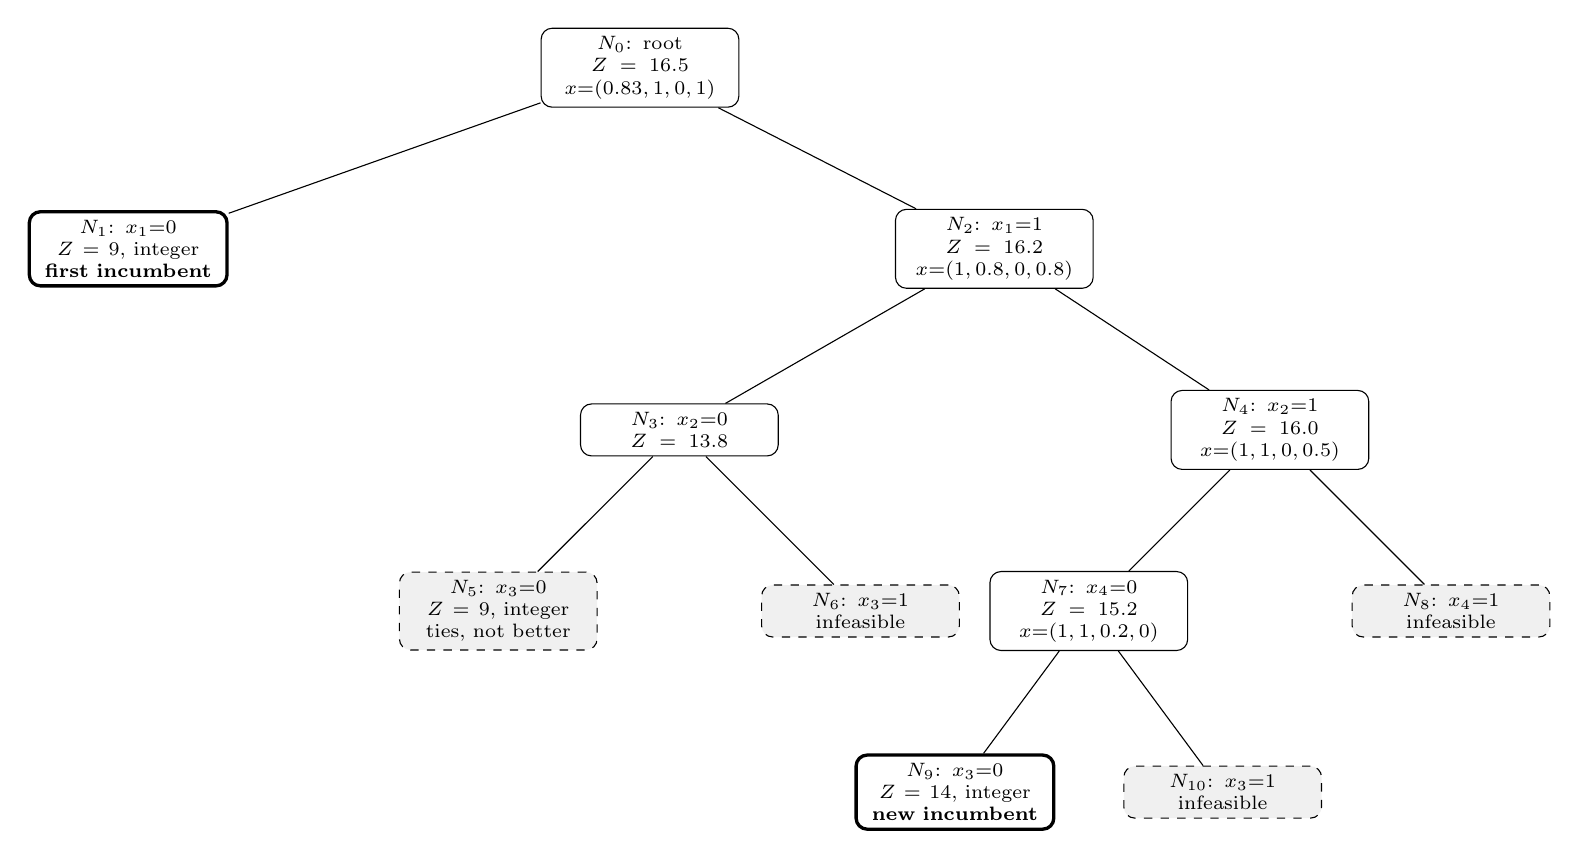
\begin{tikzpicture}[
  every node/.style={font=\scriptsize, text width=2.3cm, align=center},
  box/.style={draw, rectangle, rounded corners, inner sep=3pt},
  fathom/.style={box, dashed, fill=gray!12},
  incumbent/.style={box, very thick}
]
\node[box] (N0) at (0,0) {$N_0$: root\\$Z=16.5$\\$x{=}(0.83,1,0,1)$};

\node[incumbent] (N1) at (-6.5,-2.3) {$N_1$: $x_1{=}0$\\$Z=9$, integer\\\textbf{first incumbent}};
\node[box] (N2) at (4.5,-2.3) {$N_2$: $x_1{=}1$\\$Z=16.2$\\$x{=}(1,0.8,0,0.8)$};

\node[box] (N3) at (0.5,-4.6) {$N_3$: $x_2{=}0$\\$Z=13.8$};
\node[box] (N4) at (8,-4.6) {$N_4$: $x_2{=}1$\\$Z=16.0$\\$x{=}(1,1,0,0.5)$};

\node[fathom] (N5) at (-1.8,-6.9) {$N_5$: $x_3{=}0$\\$Z=9$, integer\\ties, not better};
\node[fathom] (N6) at (2.8,-6.9) {$N_6$: $x_3{=}1$\\infeasible};

\node[box] (N7) at (5.7,-6.9) {$N_7$: $x_4{=}0$\\$Z=15.2$\\$x{=}(1,1,0.2,0)$};
\node[fathom] (N8) at (10.3,-6.9) {$N_8$: $x_4{=}1$\\infeasible};

\node[incumbent] (N9) at (4.0,-9.2) {$N_9$: $x_3{=}0$\\$Z=14$, integer\\\textbf{new incumbent}};
\node[fathom] (N10) at (7.4,-9.2) {$N_{10}$: $x_3{=}1$\\infeasible};

\draw (N0) -- (N1);
\draw (N0) -- (N2);
\draw (N2) -- (N3);
\draw (N2) -- (N4);
\draw (N3) -- (N5);
\draw (N3) -- (N6);
\draw (N4) -- (N7);
\draw (N4) -- (N8);
\draw (N7) -- (N9);
\draw (N7) -- (N10);
\end{tikzpicture}%
}
\caption{Branch-and-bound tree for the aquaculture location problem, explored in the order $x_j=0$ before $x_j=1$ at each split. Dashed nodes are fathomed without becoming (or replacing) the incumbent; bold nodes mark the incumbent at the point it is set.}
\label{fig:bnb-tree}
\end{figure}

The result is a useful reminder that a positive individual NPV --- both
factory options have one --- does not guarantee inclusion in the optimal
solution once a shared budget constraint is taken into consideration. Both factories
compete for the same 10 mEUR, and the second farm
wins.

\section{Application: fleet renewal and retrofit under a tightening emissions cap}
\label{sec:fleet-retrofit}

\subsection{Problem context}

Before we go onto specific regulatory schemes, we will first just consider a generic set of requirements that implies that a fleet's total emissions must decline against a schedule that tightens overall emissions year on year. A shipowner facing such a
schedule can respond, per vessel, by retrofitting an emission-abatement
technology or by replacing the vessel outright with a lower-emission
newbuild. The latter can, for simplicity, be modelled as a retrofit with a 100\%
reduction and a correspondingly larger investment cost, so a single
formulation covers both (assuming replacemnt with a similar vessel). The owner must decide what
abatement technology to install on which ship, and in what time period, balancing an installation cost against an annual operating
cost and an emissions benefits to comply with the fleet-wide cap that becomes
stricter every year.

\subsection{A first formulation}
\label{sec:fleet-model-v1}

\medskip
\noindent\textbf{Sets}
\begin{align*}
  V & &&\text{vessels in the fleet, indexed by } v \\
  A & &&\text{available emission-abatement options, indexed by } a \\
  T & &&\text{time periods in the planning horizon, indexed by } t
\end{align*}

\noindent\textbf{Parameters}
\begin{align*}
  E_v & &&\text{emissions of vessel } v \text{ with no abatement installed} \\
  \gamma_a & &&\text{emission-reduction fraction achieved by option } a \\
  C_a^I & &&\text{installation cost of option } a \\
  C_a^O & &&\text{annual operating cost of option } a, \text{once installed} \\
  E_t^{\text{TOT}} & &&\text{fleet-wide allowed emissions in period } t
\end{align*}

\noindent\textbf{Variables}
\begin{align*}
  x_{vat}\in\{0,1\} & &&1 \text{ if option } a \text{ is installed on vessel } v \text{ in period } t \\
  y_{vat}\in\{0,1\} & &&1 \text{ if option } a \text{ is in use on vessel } v \text{ in period } t
\end{align*}

\noindent\textbf{Model}
\begin{align}
  \min \quad & \sum_{v\in V}\sum_{a\in A}\sum_{t\in T} \left(C_a^I x_{vat} + C_a^O y_{vat}\right) \label{eq:fleet-obj}\\
  \text{s.t.} \quad
  & \sum_{v\in V}\left(E_v - \sum_{a\in A}\gamma_a E_v y_{vat}\right) \leq E_t^{\text{TOT}}, && t \in T \label{eq:fleet-c1}\\
  & \sum_{t\in T} x_{vat} \leq 1, && v\in V, a\in A \label{eq:fleet-c2}\\
  & M\sum_{t\in T}x_{vat} \geq \sum_{t\in T}y_{vat}, && v\in V, a\in A \label{eq:fleet-c3}\\
  & y_{vat} \geq x_{vat}, && v\in V, a\in A, t\in T \label{eq:fleet-c4}\\
  & y_{vat} \geq y_{va,t-1}, && v\in V, a\in A, t\in T\setminus\{0\} \label{eq:fleet-c5}\\
  & y_{vat} - y_{va,t-1} = x_{vat}, && v\in V, a\in A, t\in T\setminus\{0\} \label{eq:fleet-c6}\\
  & x_{va,N-1} = 0, && v\in V, a\in A \label{eq:fleet-c7}\\
  & x_{vat}, y_{vat} \in \{0,1\}, && v\in V, a\in A, t\in T. \notag
\end{align}

Constraint \eqref{eq:fleet-c1} is the emissions cap. \eqref{eq:fleet-c2}
allows each option to be installed on each vessel at most once.
\eqref{eq:fleet-c3} is a big-M linking constraint, using the constructs of
Section~\ref{sec:binary-modelling}: because \eqref{eq:fleet-c2} already
forces $\sum_t x_{vat}\in\{0,1\}$, this says that $y_{vat}$ can only be
positive in \emph{some} period if $a$ is installed on $v$ in \emph{some}
period. \eqref{eq:fleet-c4} forces use to start no later than
installation. \eqref{eq:fleet-c5} forces use, once started, to persist.
\eqref{eq:fleet-c6} ties the two together in every period after the
first: use switches on ($y_{vat}=1$ while $y_{va,t-1}=0$) exactly when
installation happens ($x_{vat}=1$). \eqref{eq:fleet-c7} disallows
installing anything in the final period, since there would be no
operating periods left to recover the cost.

\subsection{A worked instance}
\label{sec:fleet-worked}

\begin{lstlisting}[language=Python]
import xpress as xp
import pandas as pd

def fleet_retrofit_model(dfV, dfA, dfT, bigM=1000):
    V, A, T = dfV.index, dfA.index, dfT.index

    x = {(v,a,t): xp.var(vartype=xp.binary, name=f"x_{v}_{a}_{t}")
         for v in V for a in A for t in T}
    y = {(v,a,t): xp.var(vartype=xp.binary, name=f"y_{v}_{a}_{t}")
         for v in V for a in A for t in T}

    p = xp.problem()
    p.addVariable(x, y)

    totCost = xp.Sum(dfA.C_I[a]*x[v,a,t] + dfA.C_O[a]*y[v,a,t]
                      for v in V for a in A for t in T)
    p.setObjective(totCost, sense=xp.minimize)

    # Emissions cap
    c1 = [xp.Sum(dfV.E[v] - xp.Sum(dfA.gamma[a]*dfV.E[v]*y[v,a,t] for a in A)
                 for v in V) <= dfT.E_req[t]
          for t in T]

    # Install at most once
    c2 = [xp.Sum(x[v,a,t] for t in T) <= 1 for a in A for v in V]

    # Big-M link: some use only if installed at some point
    c3 = [bigM*xp.Sum(x[v,a,t] for t in T) >= xp.Sum(y[v,a,t] for t in T)
          for a in A for v in V]

    # Use starts no later than installation
    c4 = [y[v,a,t] >= x[v,a,t] for t in T for a in A for v in V]

    # Use, once started, persists
    c5 = [y[v,a,t] >= y[v,a,t-1] for t in T[1:] for a in A for v in V]

    # Use switches on exactly when installation happens
    c6 = [y[v,a,t] - y[v,a,t-1] == x[v,a,t]
          for t in T[1:] for a in A for v in V]

    # No installation in the final period
    c7 = [x[v,a,T[-1]] == 0 for a in A for v in V]

    p.addConstraint(c1, c2, c3, c4, c5, c6, c7)
    p.solve()
    return p, x, y
\end{lstlisting}

This is a direct, one-for-one implementation of the model in
Section~\ref{sec:fleet-model-v1}. Three identical
vessels ($E_v=100$ for $v=1,2,3$) face the eight-period emissions cap in
Table~\ref{tab:fleet-cap}, tightening from 290 in period 0 (against an
unabated fleet total of 300) to 40 in the final period, and choose among
the three abatement options in Table~\ref{tab:fleet-options}.

\begin{table}[htbp]
\centering
\caption{Abatement option data for the worked fleet instance.}
\label{tab:fleet-options}
\begin{tabular}{@{}lccc@{}}
\toprule
Option & $\gamma_a$ & $C_a^I$ & $C_a^O$ \\
\midrule
$a_1$ & 0.3 & 20 & 3 \\
$a_2$ & 0.5 & 40 & 4 \\
$a_3$ & 1.0 & 110 & 5 \\
\bottomrule
\end{tabular}
\end{table}

\begin{table}[htbp]
\centering
\caption{Fleet-wide emissions cap by period.}
\label{tab:fleet-cap}
\begin{tabular}{@{}ccccccccc@{}}
\toprule
$t$ & 0 & 1 & 2 & 3 & 4 & 5 & 6 & 7 \\
\midrule
$E_t^{\text{TOT}}$ & 290 & 280 & 260 & 200 & 150 & 120 & 80 & 40 \\
\bottomrule
\end{tabular}
\end{table}

\begin{lstlisting}[language=Python]
dfV = pd.DataFrame({'E': [100, 100, 100]}, index=['v1','v2','v3'])
dfA = pd.DataFrame({'gamma': [0.3, 0.5, 1.0],
                     'C_I':   [20, 40, 110],
                     'C_O':   [3, 4, 5]}, index=['a1','a2','a3'])
dfT = pd.DataFrame({'E_req': [290,280,260,200,150,120,80,40]})

p, x, y = fleet_retrofit_model(dfV, dfA, dfT)
print("Total cost:", p.getObjVal())
\end{lstlisting}

Table~\ref{tab:fleet-result} gives the resulting schedule, solved to
proven optimality and cross-checked with an independent MILP solve
outside Xpress before being written up here.

\begin{table}[htbp]
\centering
\caption{Optimal installation and cost schedule for the worked instance (total cost 309).}
\label{tab:fleet-result}
\begin{tabular}{@{}cp{0.28\textwidth}rrrrr@{}}
\toprule
$t$ & Installed & $C_a^I$ & $C_a^O$ & Emissions & $E_t^{\text{TOT}}$ & Period cost \\
\midrule
0 & $a_3$ on $v_1$ & 110 & 5 & 200 & 290 & 115 \\
1 & --- & 0 & 5 & 200 & 280 & 5 \\
2 & --- & 0 & 5 & 200 & 260 & 5 \\
3 & --- & 0 & 5 & 200 & 200 & 5 \\
4 & $a_2$ on $v_2$ & 40 & 9 & 150 & 150 & 49 \\
5 & $a_1$ on $v_2$ & 20 & 12 & 120 & 120 & 32 \\
6 & $a_1,a_2$ on $v_3$ & 60 & 19 & 40 & 80 & 79 \\
7 & --- & 0 & 19 & 40 & 40 & 19 \\
\bottomrule
\end{tabular}
\end{table}

Total cost over the horizon is 309, reached by fully decarbonizing one
vessel early (period 0, since the cap tightens fastest relative to
installed capability there) and layering cheaper, partial-reduction
options onto the remaining vessels only as the cap forces it. Because all
three vessels are identical in this instance, the model is symmetric in
$v$, and any permutation of vessel labels in the schedule above is an
equally optimal alternative --- a common feature of fleet problems with
interchangeable units, and one reason real fleet models often add a
symmetry-breaking constraint (for instance, considering vessels in a
fixed order of preference) purely to speed up the solve, without changing
the achievable cost.

Figure~\ref{fig:fleet-result} plots the schedule: investment and
operating cost as stacked bars, against actual and required fleet
emissions as lines. The cap is met with zero slack in periods 3 and 7 and
by a comfortable margin elsewhere, reflecting that abatement options come
in discrete increments and cannot be timed to track a continuous cap
exactly.

\begin{figure}[htbp]
\centering

\includegraphics[width=0.75\textwidth]{ch_integer_programming/fleet_retrofit_result.png}
\caption{Cost and emissions over the planning horizon for the worked fleet retrofit instance. Bars: investment (light green) and operating cost (dark green). Lines: required cap (orange) and actual fleet emissions (blue).}
\label{fig:fleet-result}
\end{figure}

\section{Comparing maritime decarbonization regulations: CII, EU ETS, and FuelEU Maritime}
\label{sec:regimes}

To make the situation slightly more complex, a shipowner faces several regulatory instruments at the same time, each with a 
different underlying principle and structure. Here we will focus on three
regulatory instruments that currently applies (from a European perspective): the IMO's Carbon Intensity Indicator (CII), the EU
Emissions Trading System (EU ETS) as extended to shipping, and FuelEU
Maritime itself. Each measures something different, on a different
emissions basis, and enforces itself through a different mechanism.
Understanding that difference is
the point of this section. We will discuss and build each regiulatory regime's model separately.

\subsection{Three different regulatory logics}
\label{sec:regimes-logics}

Table~\ref{tab:regime-comparison} summarises the three instruments along
the dimensions that matter for modelling them: what they measure, on
which emissions basis, and how non-compliance is enforced.

\begin{table}[htbp]
\centering
\caption{Three overlapping maritime decarbonization instruments.}
\label{tab:regime-comparison}
\begin{tabular}{@{}p{0.14\textwidth}p{0.24\textwidth}p{0.16\textwidth}p{0.34\textwidth}@{}}
\toprule
Instrument & What it measures & Basis & Enforcement \\
\midrule
CII & CO2 per unit of transport work (an \emph{efficiency} metric) & Tank-to-wake (TtW) & Letter rating (A--E); rating-based operational and commercial consequences, no direct fine \\
EU ETS & Total CO2 emitted (an \emph{absolute} quantity) & Tank-to-wake (TtW) & Carbon price paid on every tonne, phased in \\
FuelEU Maritime & GHG intensity of energy used (an \emph{intensity} metric) & Well-to-wake (WtW) & Fixed penalty rate on any shortfall against a tightening target \\
\bottomrule
\end{tabular}
\end{table}

The \textit{Basis} is important to take into account. \emph{Tank-to-wake} (TtW)
counts only the CO2 released when the fuel is burned onboard.
\emph{Well-to-wake} (WtW) additionally includes the emissions from
producing and transporting the fuel before it reaches the ship. This is important. FOr instance, 
the CO2 released when burning a biogenic fuel such as
bio-methanol is counted as zero at the tank-to-wake stage, since that
carbon was recently absorbed from the atmosphere by the feedstock; it is
only the WtW basis that carries the fuel's production-stage footprint. A
fuel switch that looks like a complete solution under a TtW-based regime
can therefore be only a partial one under a WtW-based regime. A
second difference is structural rather than accounting-based: CII and
FuelEU both compare an attained value against a target and act only on
the shortfall, while EU ETS charges for every tonne regardless of any
target at all.

\subsection{A very simplified model for illustration}
\label{sec:regimes-setting}

For the regulatory comparison we consider only a single representative
vessel rather than a fleet, choosing a blend of two fuels each period: the incumbent HFO, and
bio-methanol.

\medskip
\noindent\textbf{Sets}: $K=\{\text{HFO},\text{bio}\}$, candidate fuels.

\medskip
\noindent\textbf{Parameters}
\begin{align*}
  Q &&& \text{the vessel's annual energy consumption (GJ), fixed} \\
  TW &&& \text{the vessel's annual transport work (tonne-nautical miles), fixed} \\
  g_k^{\text{TtW}} &&& \text{tank-to-wake CO2 intensity of fuel } k \text{ (gCO2/MJ)} \\
  g_k^{\text{WtW}} &&& \text{well-to-wake GHG intensity of fuel } k \text{ (gCO2e/MJ)} \\
  c_k &&& \text{cost of fuel } k \text{ (EUR/GJ)}
\end{align*}

\noindent\textbf{Core variable}, shared by every model in this section:
\begin{align*}
  x_{kt}\in[0,1] &&& \text{share of energy met by fuel } k \text{ in period } t, \quad \sum_{k\in K}x_{kt}=1.
\end{align*}

Table~\ref{tab:regime-fuels} gives the data used throughout. HFO's TtW
value follows from IMO Annex VI's carbon factor for heavy fuel oil
($C_F=3.114$~gCO2/g fuel) and a representative lower heating value; its
WtW value is FuelEU's own reference intensity, so the difference between
the two ($13.7$~gCO2/MJ) is HFO's upstream, well-to-tank footprint.
Bio-methanol's TtW value is zero under the biogenic-carbon convention
just described; its WtW value of $32.2$~gCO2e/MJ is the production-stage
footprint reported by \citet{cho2027}. Fuel costs are illustrative.

\begin{table}[htbp]
\centering
\caption{Fuel data used throughout this section.}
\label{tab:regime-fuels}
\begin{tabular}{@{}lccc@{}}
\toprule
Fuel & $g_k^{\text{TtW}}$ (gCO2/MJ) & $g_k^{\text{WtW}}$ (gCO2e/MJ) & $c_k$ (EUR/GJ) \\
\midrule
HFO & 77.4 & 91.16 & 15 \\
Bio-methanol & 0.0 & 32.2 & 38 \\
\bottomrule
\end{tabular}
\end{table}

The vessel consumes $Q=10{,}000$~GJ/yr and produces
$TW=75{,}000{,}000$~tonne-nautical miles/yr, giving it a tank-to-wake
attained CII of $77.4\times Q\times1000/TW=10.32$~gCO2/tonne-nm and total
TtW emissions of $774$~tonnes CO2/yr while burning pure HFO --- the
common starting point for every sub-model below.

\subsection{The Carbon Intensity Indicator (CII)}
\label{sec:regimes-cii}

CII compares a vessel's attained carbon intensity,
$\sum_k g_k^{\text{TtW}}x_{kt}\,Q\,1000/TW$ (gCO2/tonne-nm), against a
required value that tightens each year by a fixed reduction factor $r_t$
off a 2019 reference intensity $I^{\text{CII}}_{\text{ref}}$. In
practice a vessel that misses its required value receives a worse letter
rating (D or E) and must file a corrective action plan; there is no
direct fine. We model the commercial consequence of a worse rating, such as
higher financing or insurance cost, a weaker position when chartering, as a 
cost $c^{\text{CII}}$ per tonne of the implied shortfall, making
clear that this is a modelled proxy for an indirect consequence, not a
regulatory payment. In a comprehensive model, the CII may be modelled simply as 
constraints that partly reflects the requirements, and partly company policy/strategy.

\begin{align}
  \min \quad & \sum_{k\in K}c_kx_{kt}\,Q + c^{\text{CII}}s_t^{\text{CII}} \notag\\
  \text{s.t.} \quad & s_t^{\text{CII}} \geq \left(\sum_{k\in K}g_k^{\text{TtW}}x_{kt}\,\frac{Q}{1000} - I^{\text{CII}}_t\,\frac{TW}{10^6}\right), \notag\\
  & \qquad I^{\text{CII}}_t = I^{\text{CII}}_{\text{ref}}(1-r_t) \notag\\
  & \sum_{k\in K}x_{kt}=1, \quad x_{kt}\geq0,\ s_t^{\text{CII}}\geq0. \notag
\end{align}

Using $I^{\text{CII}}_{\text{ref}}=10$~gCO2/tonne-nm and the IMO's
confirmed reduction factors (Table~\ref{tab:cii-factors}), solving this
for each of 2023--2026 gives $x_{\text{bio},t}=0$ throughout, at a
soft-consequence rate of $c^{\text{CII}}=50$~EUR/tonne: the extra fuel
cost of a full switch (EUR~230{,}000/yr) far exceeds even the largest
possible rating consequence (at most
$774\times50=$~EUR~38{,}700/yr, reached only if the required value fell
to zero). A rational owner, at this consequence rate, would simply
accept the worse rating and file the paperwork.

\begin{table}[htbp]
\centering
\caption{IMO CII reduction factors and implied required intensity (illustrative reference intensity of 10 gCO2/tonne-nm).}
\label{tab:cii-factors}
\begin{tabular}{@{}ccc@{}}
\toprule
Year & Reduction factor $r_t$ & Required CII (gCO2/tonne-nm) \\
\midrule
2023 & 5\% & 9.50 \\
2024 & 7\% & 9.30 \\
2025 & 9\% & 9.10 \\
2026 & 11\% & 8.90 \\
\bottomrule
\end{tabular}
\end{table}

\subsection{The EU Emissions Trading System (EU ETS)}
\label{sec:regimes-ets}

EU ETS is structurally simpler: there is no target and no rating, only a
price $c^{\text{CO2}}$ paid on every tonne of TtW CO2 emitted, phased in
at a fraction $\phi_t$ of full scope (Table~\ref{tab:ets-phasein}).

\begin{align}
  \min \quad & \sum_{k\in K}c_kx_{kt}\,Q + \phi_t\,c^{\text{CO2}}\sum_{k\in K}g_k^{\text{TtW}}x_{kt}\,\frac{Q}{1000} \notag\\
  \text{s.t.} \quad & \sum_{k\in K}x_{kt}=1, \quad x_{kt}\geq0. \notag
\end{align}

\begin{table}[htbp]
\centering
\caption{EU ETS phase-in for shipping.}
\label{tab:ets-phasein}
\begin{tabular}{@{}ccc@{}}
\toprule
2024 & 2025 & 2026 onward \\
\midrule
40\% & 70\% & 100\% \\
\bottomrule
\end{tabular}
\end{table}

At today's allowance price of roughly $c^{\text{CO2}}=80$~EUR/tonne,
solving this gives $x_{\text{bio},t}=0$ in every period too: the price
needed to make a full switch worthwhile is, mechanically,
$230{,}000/774\approx297$~EUR/tonne --- almost four times today's price
--- and this threshold is the \emph{same} number that appeared in the
CII sub-model, because both instruments price the same TtW quantity, and
switching fuel changes that quantity the same way regardless of which
instrument is doing the pricing. What differs between the two regimes is
not the price needed to trigger switching, but how much of the vessel's
emissions get priced at all once that threshold is reached: EU ETS
prices every tonne, all the time; CII only prices the shortfall against
a rating.

\subsection{FuelEU Maritime}
\label{sec:regimes-fueleu}

FuelEU compares WtW intensity, not TtW, against its own target
(Table~\ref{tab:fueleu-target-recap}), and its shortfall is priced at a
fixed, deliberately punitive rate --- this is the baseline model of
Section~\ref{sec:fleet-model-v1}, applied to a single vessel:

\begin{align}
  \min \quad & \sum_{k\in K}c_kx_{kt}\,Q + c^{\text{pen}}s_t^{\text{FuelEU}} \notag\\
  \text{s.t.} \quad & s_t^{\text{FuelEU}} \geq \left(\sum_{k\in K}g_k^{\text{WtW}}x_{kt} - I_t^{\text{tar}}\right)\frac{Q}{1000}, \notag\\
  & \sum_{k\in K}x_{kt}=1, \quad x_{kt}\geq0,\ s_t^{\text{FuelEU}}\geq0. \notag
\end{align}

\begin{table}[htbp]
\centering
\caption{FuelEU Maritime target WtW GHG intensity by milestone year.}
\label{tab:fueleu-target-recap}
\begin{tabular}{@{}cccccccc@{}}
\toprule
Year & 2025 & 2030 & 2035 & 2040 & 2045 & 2050 \\
\midrule
$I_t^{\text{tar}}$ (gCO2e/MJ) & 89.34 & 85.69 & 77.95 & 62.90 & 34.64 & 18.23 \\
\bottomrule
\end{tabular}
\end{table}

At $c^{\text{pen}}=700$~EUR/tonne --- well above the 297--390~EUR/tonne
range needed to make switching worthwhile on either basis --- this
regime, and only this one, drives genuine, gradual switching on its own,
shown in Table~\ref{tab:fueleu-solo-recap}: from a token 3\% blend in
2025 to full bio-methanol by 2050, at which point a residual deficit
remains, because bio-methanol's WtW intensity (32.2) still exceeds the
2050 target (18.23). This is exactly the FuelEU behaviour reported in
Section~\ref{sec:fleet-retrofit}, now for a single vessel instead of a
fleet.

\begin{table}[htbp]
\centering
\caption{FuelEU-only optimal bio-methanol share.}
\label{tab:fueleu-solo-recap}
\begin{tabular}{@{}ccccccc@{}}
\toprule
Year & 2025 & 2030 & 2035 & 2040 & 2045 & 2050 \\
\midrule
Bio-methanol share & 3.1\% & 9.3\% & 22.4\% & 47.9\% & 95.9\% & 100\% \\
\bottomrule
\end{tabular}
\end{table}

\subsection{A shipowner facing all three: the combined model}
\label{sec:regimes-combined}

None of the three regimes is optional, so the model a shipowner actually
needs combines all three cost terms over the same fuel choice:

\begin{align}
  \min \quad & \sum_{k\in K}c_kx_{kt}\,Q
    + c^{\text{CII}}s_t^{\text{CII}}
    + \phi_t\,c^{\text{CO2}}\sum_{k\in K}g_k^{\text{TtW}}x_{kt}\,\frac{Q}{1000}
    + c^{\text{pen}}s_t^{\text{FuelEU}} \notag\\
  \text{s.t.} \quad & s_t^{\text{CII}} \geq \left(\sum_{k\in K}g_k^{\text{TtW}}x_{kt}\,\frac{Q}{1000} - I^{\text{CII}}_t\,\frac{TW}{10^6}\right) \notag\\
  & s_t^{\text{FuelEU}} \geq \left(\sum_{k\in K}g_k^{\text{WtW}}x_{kt} - I_t^{\text{tar}}\right)\frac{Q}{1000} \notag\\
  & \sum_{k\in K}x_{kt}=1, \quad x_{kt}\geq0,\ s_t^{\text{CII}},s_t^{\text{FuelEU}}\geq0. \notag
\end{align}

Nothing here is new modelling machinery --- it is literally the union of
the three constraint sets above, added to one objective --- which is the
point: once each regime has its own clean model, combining them is
bookkeeping, not new theory. Solving it, using an illustrative
extrapolation of the CII reduction factor beyond 2026 consistent with
the IMO's 2023 GHG Strategy checkpoints (at least 20\% by 2030, 70\% by
2040, net-zero by 2050, relative to a 2008 reference; ship-specific
factors beyond 2026 have not actually been set), gives the bio-methanol
share in Table~\ref{tab:fueleu-solo-recap} again, \emph{unchanged}, in
every period.

That is a real finding, not a modelling coincidence, and worth
explaining rather than just reporting. Section~\ref{sec:regimes-ets}
already showed that CII and EU ETS, at realistic price levels, cannot
justify switching on their own; adding their costs on top of FuelEU
changes the bill, not the strategy, because FuelEU's own 700~EUR/tonne
rate is already high enough to be the sole driver of the fuel choice ---
CII and EU ETS mostly come along for the ride. They are not free riders,
though: Figure~\ref{fig:regime-comparison} plots the fuel strategy each
regime would choose in isolation, and Table~\ref{tab:regime-cost}
prices out what it would cost to actually \emph{follow} the CII/EU
ETS-optimal strategy (pure HFO, since neither justifies switching alone)
once all three regulations' bills come due on it, against the true joint
optimum.

\begin{figure}[htbp]
\centering

\includegraphics[width=0.7\textwidth]{ch_integer_programming/regime_comparison.png}
\caption{Optimal bio-methanol share under each regime considered in isolation.}
\label{fig:regime-comparison}
\end{figure}

\begin{table}[htbp]
\centering
\caption{Total 2025--2050 cost under the three regulations, by strategy.}
\label{tab:regime-cost}
\begin{tabular}{@{}lr@{}}
\toprule
Strategy & Total cost (EUR) \\
\midrule
Pure HFO (the CII- and EU ETS-optimal choice) & 2{,}629{,}114 \\
Joint optimum (identical to the FuelEU-only strategy) & 1{,}844{,}434 \\
\bottomrule
\end{tabular}
\end{table}

Optimizing only for the two regimes that, individually, never justify
switching costs an extra EUR~785{,}000 over the horizon --- a
43\% premium --- once FuelEU's bill for the same choice is added in. The
general lesson is not ``switch fuels''; it is that a shipowner facing
several overlapping regulations needs to identify which one is actually
\emph{binding} the strategy (here, FuelEU, by design: its rate was set
well above prevailing carbon prices specifically so it would not need
the other two to work) and which are along for the ride, rather than
optimizing against each in isolation and hoping they add up.

The other half of the lesson is the one flagged in
Section~\ref{sec:regimes-logics}: a shipowner who tracked \emph{only}
CII and EU ETS could reasonably conclude that a full switch to
bio-methanol solves everything, since it drives tank-to-wake emissions
to zero. Table~\ref{tab:fueleu-solo-recap} shows that this is not true
under FuelEU: the same fuel, evaluated on a well-to-wake basis, leaves a
persistent shortfall from 2050 onward. Three different regulations,
looking at the same ship and the same fuel, can reach three different
verdicts on how well it is doing --- and a strategy built for one basis
is not automatically a strategy for the others.

Two extensions are natural from here, both left as exercises rather than
developed further. First, FuelEU's own intertemporal flexibility ---
banking a surplus, borrowing against a future one, or pooling compliance
across a fleet's vessels --- can be layered onto its sub-model above
using exactly the constructs of Table~\ref{tab:binary-constructs};
neither CII nor EU ETS, as modelled here, has anything to bank, since
neither carries a balance from one period to the next. Second, CII's
denominator, transport work, has so far been held fixed; the production-function
framework used for ship size and speed earlier in this course is exactly the tool
needed to let speed --- and hence both fuel consumption and transport work
simultaneously --- become a decision variable instead of a parameter,
coupling CII compliance directly to the speed-and-size problem this
course opened with.


